\chapter{Part 4c. Instruction Level Parallelism}
In the last chapter, we've seen how pipelining can make it easier to parallelize indepent operations making it the overall process faster.

\subsection{Pipelining the Processor}
Pipelining in processors is a technique that splits the execution of an instruction into multiple stages, each handled in parallel by separate hardware units. By doing so, multiple instructions can be processed simultaneously, thereby increasing the overall throughput of the processor without increasing the clock frequency.

\begin{itemize}
    \item \textbf{Fetch (F)}: Retrieve the instruction from memory (often from the instruction cache).
    \item \textbf{Decode (D)}: Interpret the fetched instruction, identify operands, and configure the control signals for execution.
    \item \textbf{Execute (E)}: Perform the required operations (e.g., arithmetic, logic, load, store).
\end{itemize}

\noindent In a basic pipeline with three stages (F, D, E), each stage takes one clock cycle. While one instruction is being executed, a second instruction can be decoded, and a third can be fetched at the same time. This overlapping of tasks leads to a substantial improvement in instruction throughput.

%\begin{figure}[htbp]
%    \centering
%    % Replace 'placeholder_image1.png' with your actual figure file
%    \includegraphics[width=0.7\textwidth]{placeholder_image1.png}
%    \caption{Conceptual view of a three-stage pipeline. Each instruction proceeds through Fetch, Decode, and Execute stages in order.}
%    \label{fig:basic-pipeline}
%\end{figure}

\subsubsection*{Example Pipeline Schedule}
Consider a schedule where three instructions (\(i\), \(i+1\), and \(i+2\)) enter the pipeline. Each instruction occupies a unique pipeline stage in any given clock cycle. Figure~\ref{fig:pipeline-schedule} illustrates how each instruction advances one stage every cycle:
\[
\begin{array}{c|cccccc}
\text{Time} & t & t+1 & t+2 & t+3 & t+4 & t+5 \\ \hline
i     & F & D & E & - & - & - \\
i+1   & - & F & D & E & - & - \\
i+2   & - & - & F & D & E & - \\
\end{array}
\]

%\begin{figure}[htbp]
%    \centering
%    % Replace 'placeholder_image2.png' with your actual figure file
%    \includegraphics[width=0.7\textwidth]{placeholder_image2.png}
%    \caption{A pipeline schedule showing instruction overlap in each stage.}
%    \label{fig:pipeline-schedule}
%\end{figure}

\subsubsection*{Multi-Cycle Processor vs.\ Pipelined Processor}
A \emph{multi-cycle} processor might use multiple cycles to execute every instruction (e.g., separate cycles for Fetch, Decode, ALU, Memory Access, and Write Back), but only one instruction flows through the processor at a time. In contrast, a \emph{pipelined} processor allows the next instruction to begin its Fetch stage in parallel with the Decode stage of the previous instruction, greatly improving throughput.
\begin{center}
    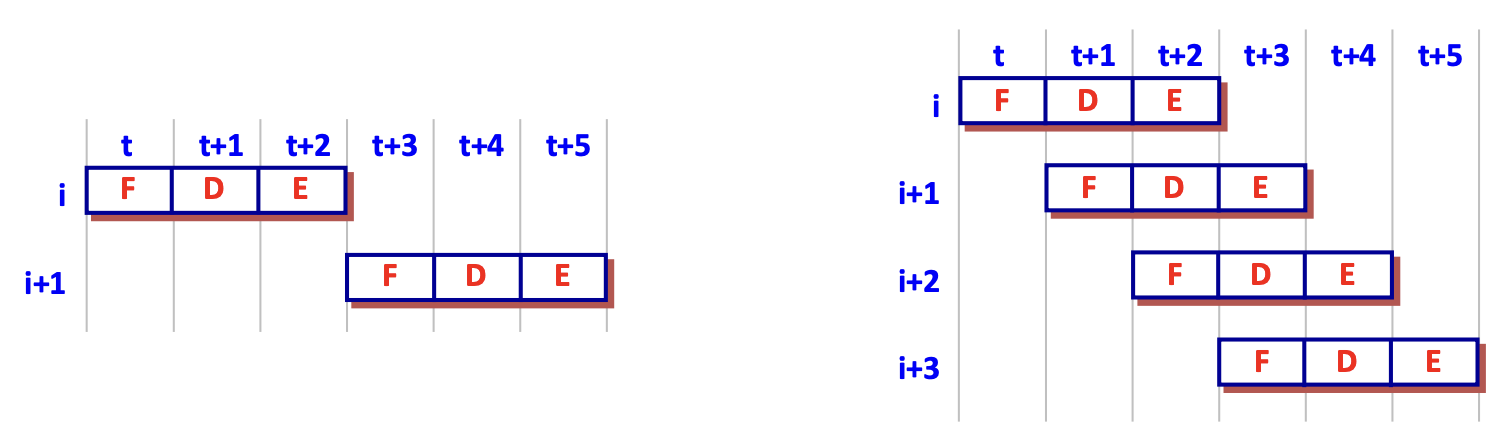
\includegraphics[width=0.65\textwidth]{chapters/chapter4c/images/vs.png}
\end{center}
\subsubsection*{Key Observations for Pipelining}
\begin{enumerate}
    \item \textbf{Repetitive Activity}: Pipelining is effective only when the processor has a large number of instructions to execute.
    \item \textbf{Subactivities}: Each major task (Fetch, Decode, Execute, etc.) should be clearly separable into sub-stages to allow parallel operation.
    \item \textbf{Throughput Gain}: Once the pipeline is full, an instruction completes at the end of every cycle (in the ideal case), increasing throughput.
\end{enumerate}

\noindent Properly designing pipeline stages and handling hazards (such as data, control, and structural hazards) ensures that the pipeline delivers high performance without correctness issues.

\section{Hardware Reuse Across Processor Stages}

In processor design, the approach to hardware reuse varies significantly between multicycle and pipelined architectures. Understanding these differences is crucial for optimizing performance and resource utilization.

\subsection{Multicycle Processor Architecture}

A multicycle processor divides instruction execution into distinct \textbf{states}, allowing certain hardware components to be shared across these states. This sharing is feasible because the components are not required simultaneously, enabling efficient resource utilization.

\begin{itemize}
    \item \textbf{FETCH} State: Typically involves an \textit{adder} to increment the program counter (PC).
    \item \textbf{EXECUTE} State: Requires an \textit{Arithmetic Logic Unit} (ALU) to perform operations.
\end{itemize}

Since the \textit{adder} and the \textit{ALU} are not active concurrently, the ALU can be repurposed to increment the PC during the FETCH state. This reuse reduces the overall hardware complexity and cost.

\subsection{Pipelined Processor Architecture}

In contrast, a pipelined processor operates with multiple \textbf{stages} that are active simultaneously. Each stage performs a different part of the instruction execution process, necessitating dedicated hardware for each stage to avoid conflicts and ensure seamless parallelism.

\begin{itemize}
    \item All pipeline stages are \textit{active concurrently}, handling different instructions in each stage.
    \item Hardware components cannot be shared across stages since multiple instructions require access to the same resources simultaneously.
    \item Consequently, hardware must be \textit{replicated} where necessary to maintain pipeline efficiency and prevent bottlenecks.
\end{itemize}

The inability to share hardware across pipeline stages often leads to increased hardware requirements compared to multicycle processors. However, this replication is essential for achieving high instruction throughput and maximizing pipeline performance.

\section{Two Main Challenges in Processor Design}

Designing efficient processors involves addressing several challenges. Two prominent issues are the \textbf{CISC vs. RISC} debate and \textbf{instruction independence}.

\subsection{CISC vs. RISC}

\begin{enumerate}
    \item \textbf{Pipeline Efficiency in CISC vs. RISC}
    \begin{itemize}
        \item \textbf{Question}: Can we construct a pipeline for a Complex Instruction Set Computer (CISC) that matches the efficiency of a pipeline designed for a Reduced Instruction Set Computer (RISC)?
        \item \textbf{Implications}:
        \begin{itemize}
            \item RISC architectures typically use simpler, fixed-length instructions, which are easier to pipeline efficiently.
            \item CISC architectures have more complex, variable-length instructions, potentially complicating pipeline design and reducing efficiency.
            \item The distinction influences processor complexity, performance, and power consumption.
        \end{itemize}
    \end{itemize}
\end{enumerate}

Understanding the trade-offs between CISC and RISC is essential for making informed decisions about processor design, balancing factors such as instruction complexity, pipeline efficiency, and overall performance.

\subsection{Instruction Independence}

\begin{enumerate}
    \setcounter{enumi}{1}
    \item \textbf{Ensuring Correct Execution with Dependent Instructions}
    \begin{itemize}
        \item \textbf{Issue}: Instructions are often \textit{dependent} on the results of preceding instructions, violating the assumption of \textbf{instruction independence}.
        \item \textbf{Challenge}: Executing code correctly in the presence of such dependencies requires sophisticated mechanisms to handle hazards, such as data forwarding or pipeline stalls.
        \item \textbf{Considerations}:
        \begin{itemize}
            \item Ensuring correct program behavior without sacrificing pipeline throughput.
            \item Balancing hardware complexity with the ability to maintain high instruction-level parallelism.
        \end{itemize}
    \end{itemize}
\end{enumerate}

Addressing instruction dependencies is critical for maintaining the integrity of program execution while striving for optimal pipeline performance. Techniques such as out-of-order execution and speculative execution are often employed to mitigate the impact of these dependencies.
